\documentclass[11pt]{article}
\usepackage{amsmath, amssymb, amscd, amsthm, amsfonts}
\usepackage{graphicx}
\usepackage{hyperref}
\usepackage{subfigure}
\usepackage{float}
\usepackage{rotating}
\usepackage{tikz}
\usepackage{xcolor}
\usepackage{listings}
\definecolor{vgreen}{RGB}{104,180,104}
\definecolor{vblue}{RGB}{49,49,255}
\definecolor{vorange}{RGB}{255,143,102}
\lstdefinestyle{verilog-style}
{
    language=Verilog,
    basicstyle=\small\ttfamily,
    keywordstyle=\color{vblue},
    identifierstyle=\color{black},
    commentstyle=\color{vgreen},
    numbers=left,
    numberstyle=\tiny\color{black},
    numbersep=10pt,
    tabsize=4,
    moredelim=*[s][\colorIndex]{[}{]},
    literate=*{:}{:}1
}

\makeatletter
\newcommand*\@lbracket{[}
\newcommand*\@rbracket{]}
\newcommand*\@colon{:}
\newcommand*\colorIndex{%
    \edef\@temp{\the\lst@token}%
    \ifx\@temp\@lbracket \color{black}%
    \else\ifx\@temp\@rbracket \color{black}%
    \else\ifx\@temp\@colon \color{black}%
    \else \color{vorange}%
    \fi\fi\fi
}
\makeatother

\usepackage{trace}



\oddsidemargin 0pt
\evensidemargin 0pt
\marginparwidth 40pt
\marginparsep 10pt
\topmargin -20pt
\headsep 10pt
\textheight 8.7in
\textwidth 6.65in
\linespread{1.2}

\title{Digital Bubble Level - Cadence RTL Synthesis}
\author{Vladislav Pomogaev - 26951160}
\date{October 10, 2021}

\newcommand{\rr}{\mathbb{R}}

\newcommand{\al}{\alpha}
\DeclareMathOperator{\conv}{conv}
\DeclareMathOperator{\aff}{aff}

\begin{document}

\maketitle

\section{Introduction}

\section{Outputs of RTL Compiler}

\begin{figure}[H]
    \centering
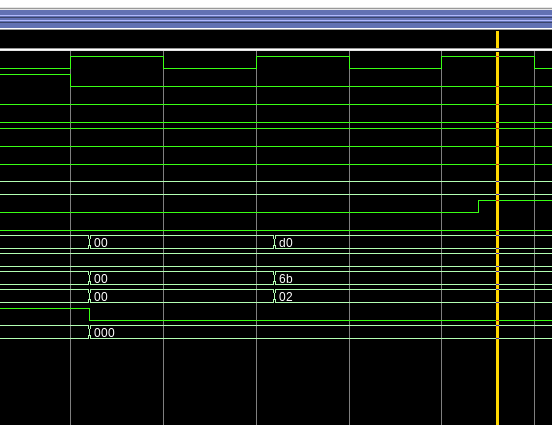
\includegraphics[width=0.99\textwidth]{closeup_delayed_wave.png}
    \caption{}
\end{figure}
\begin{figure}[H]
    \centering
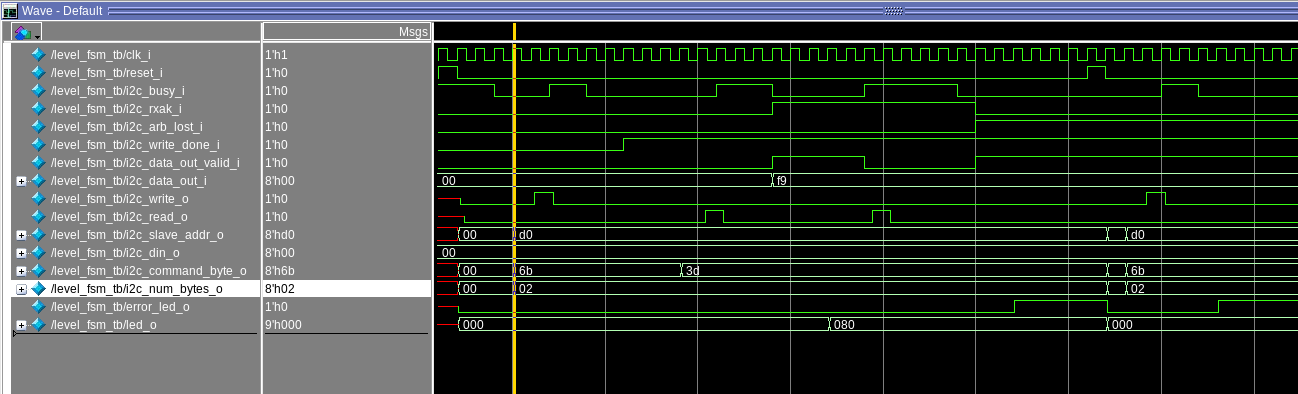
\includegraphics[width=0.99\textwidth]{delayed_wave.png}
    \caption{}
\end{figure}

\section{Outputs of RTL Compiler}
\subsection{Reports}
level{\_}fsm{\_}area.rpt
\lstinputlisting[style={}, basicstyle=\tiny,]{synth/out/level_fsm_area.rpt}
level{\_}fsm{\_}gates.rpt
\lstinputlisting[style={}, basicstyle=\tiny,]{synth/out/level_fsm_gates.rpt}
level{\_}fsm{\_}power.rpt
\lstinputlisting[style={}, basicstyle=\tiny,]{synth/out/level_fsm_power.rpt}
level{\_}fsm{\_}timing.rpt
\lstinputlisting[style={}, basicstyle=\tiny,]{synth/out/level_fsm_timing.rpt}
\subsection{Mapped Verilog}
level{\_}fsm{\_}map.v
\lstinputlisting[style={verilog-style}, basicstyle=\tiny,]{synth/out/level_fsm_map.v}

\end{document}